 %%%%%%%%%%%%%%%%%%%%%%%%%%%%%%%%%%%%%%%%%
% University Assignment Title Page 
% LaTeX Template
% Version 1.0 (27/12/12)
%
% This template has been downloaded from:
% http://www.LaTeXTemplates.com
%
% Original author:
% WikiBooks (http://en.wikibooks.org/wiki/LaTeX/Title_Creation)
%
% License:
% CC BY-NC-SA 3.0 (http://creativecommons.org/licenses/by-nc-sa/3.0/)
% 
% Instructions for using this template:
% This title page is capable of being compiled as is. This is not useful for 
% including it in another document. To do this, you have two options: 
%
% 1) Copy/paste everything between \begin{document} and \end{document} 
% starting at \begin{titlepage} and paste this into another LaTeX file where you 
% want your title page.
% OR
% 2) Remove everything outside the \begin{titlepage} and \end{titlepage} and 
% move this file to the same directory as the LaTeX file you wish to add it to. 
% Then add \documentclass[12pt]{article}
\usepackage[english]{babel}
\usepackage{amsmath}
\usepackage{graphicx}
\usepackage{textcomp}
\usepackage{parskip}
\usepackage[colorinlistoftodos]{todonotes}
\usepackage{csquotes}
\usepackage{float}
\usepackage[backend=biber,style=ieee]{biblatex}
\addbibresource{bibliography.bib}

\begin{document}

\begin{titlepage}

\newcommand{\HRule}{\rule{\linewidth}{0.5mm}}
\center 

\textsc{\LARGE Iowa State University }\\[1.5cm] 
\textsc{\Large Center for Statistics and Applications in Forensic
Evidence
}\\[0.5cm] 

\HRule \\[0.4cm]
{ \huge \bfseries Shoe Print Data Collection: Additional Methods }\\[0.4cm] 
\HRule \\[1.5cm]



\begin{center}
\centering
 
\includegraphics[scale=.4]{csafe-logo}\\[1cm]
\end{center}







\end{titlepage}

\section{Introduction}

 When developing the methodology for the longitudinal shoe study conducted by the Center for Statistics and Applications in Forensic Evidence (CSAFE), collection procedures were designed to obtain the most ideal shoe-sole impression possible. While these images will be useful to the researcher and practitioner communities, they do not provide realistic examples of prints that would be collected from a crime scene/suspected crime scene. For this reason, CSAFE researchers have compiled this manual which contains procedures for further data collection and offers new, or edited, procedures that better represent the practices of current forensic examiners and crime scene teams. If at any time there is a question on any of these procedures, please make a note using a post-it note and e-mail the principal investigator, the project manager, the faculty in charge of the study, or the author of the specific procedure. 

\end{document} to your LaTeX file where you want your
% title page.
%
%%%%%%%%%%%%%%%%%%%%%%%%%%%%%%%%%%%%%%%%%
%\title{Description of Outsole Impression Methods}
%----------------------------------------------------------------------------------------
%	PACKAGES AND OTHER DOCUMENT CONFIGURATIONS
%----------------------------------------------------------------------------------------

\documentclass[12pt]{article}
\usepackage[english]{babel}
\usepackage[utf8x]{inputenc}
\usepackage{amsmath}
\usepackage{graphicx}
\usepackage[colorinlistoftodos]{todonotes}

%% Forcing images to stay in their corresponding section
\usepackage{placeins}
\let\Oldsection\section
\renewcommand{\section}{\FloatBarrier\Oldsection}
\let\Oldsubsection\subsection
\renewcommand{\subsection}{\FloatBarrier\Oldsubsection}
\let\Oldsubsubsection\subsubsection
\renewcommand{\subsubsection}{\FloatBarrier\Oldsubsubsection}


% Set images path
\graphicspath{ {images/} }

% Links to sections.
\usepackage{hyperref}

\begin{document}

\begin{titlepage}

\newcommand{\HRule}{\rule{\linewidth}{0.5mm}} % Defines a new command for the horizontal lines, change thickness here

\center % Center everything on the page
 
%----------------------------------------------------------------------------------------
%	HEADING SECTIONS
%----------------------------------------------------------------------------------------
\textsc{\LARGE Iowa State University}\\[1.5cm] % Name of your university/college
\textsc{\large Center for Statistics and Applications in Forensic Evidence }\\[0.5cm] % Minor heading such as course title

%----------------------------------------------------------------------------------------
%	TITLE SECTION
%----------------------------------------------------------------------------------------

\HRule \\[0.4cm]
{ \huge \bfseries Visible Muddy Shoe Print on a Hard Surface: Procedure}\\[0.4cm] % Title of your document
\HRule \\[1.5cm]
 
%----------------------------------------------------------------------------------------
%	AUTHOR SECTION
%----------------------------------------------------------------------------------------
\begin{minipage}{0.4\textwidth}
\begin{flushleft} \large
\emph{Author:}\\
Jenny Kim, \newline Benjamin Wonderlin, and James \textsc{E. Kruse, } % Your name
\end{flushleft}
\end{minipage}
~
\begin{minipage}{0.4\textwidth}
\begin{flushright} \large
\emph{Principal Investigator:} \\
 \textsc{Dr. Guillermo Basulto-Elias, and Dr. Susan Vanderplas } % Supervisor's Name
\end{flushright}
\end{minipage}\\[2cm]

% If you don't want a supervisor, uncomment the two lines below and remove the section above
%\Large \emph{Author:}\\
%John \textsc{Smith}\\[3cm] % Your name
%----------------------------------------------------------------------------------------
%	LOGO SECTION
%----------------------------------------------------------------------------------------


\includegraphics[scale=.5]{Logo}\\[1cm]

\begin{center}
\begin{tabular}{ c   |   c } 
 
\end{tabular}
\end{center}
%----------------------------------------------------------------------------------------
%	DATE SECTION
%----------------------------------------------------------------------------------------

{\large \today}\\[2cm] % Date, change the \today to a set date if you want to be precise


 
%----------------------------------------------------------------------------------------

\vfill % Fill the rest of the page with whitespace

\end{titlepage}
 
\tableofcontents

\newpage

\section{Introduction}

The following is the recommended procedure for creating, controlled, muddy shoe prints on wood and vinyl surfaces. All care should be taken to contain any and all mud that is generated during this procedure. 

\subsection{Building the flooring paths}
Note: This is the same procedure used to create the flooring paths used in the "Dust Shoe Impression Photography and Lifting: Procedure". The materials can be used for both methods.
Note: Four 6 ft. x 1 ft. boards will be needed to create all necessary boards. 

1. To created the linoleum flooring path, lay out two 6 ft. x 1 ft. (2cm by 147cm) boards on an even surface. 

2. Peel back the adhesive from the linoleum flooring. Cover one entire board with flooring, offsetting each row from the last (think traditional flooring arrangement).

3. To created the hard wood flooring path, lay out two 6 ft. x 1 ft. (2cm by 147cm) boards on an even surface.

4. Snap together the hardwood pieces on top of the two boards (Figure 1). Screw down the corners of the hardwood into the board. (Figure 2).

\begin{figure}[!htp]
\centering
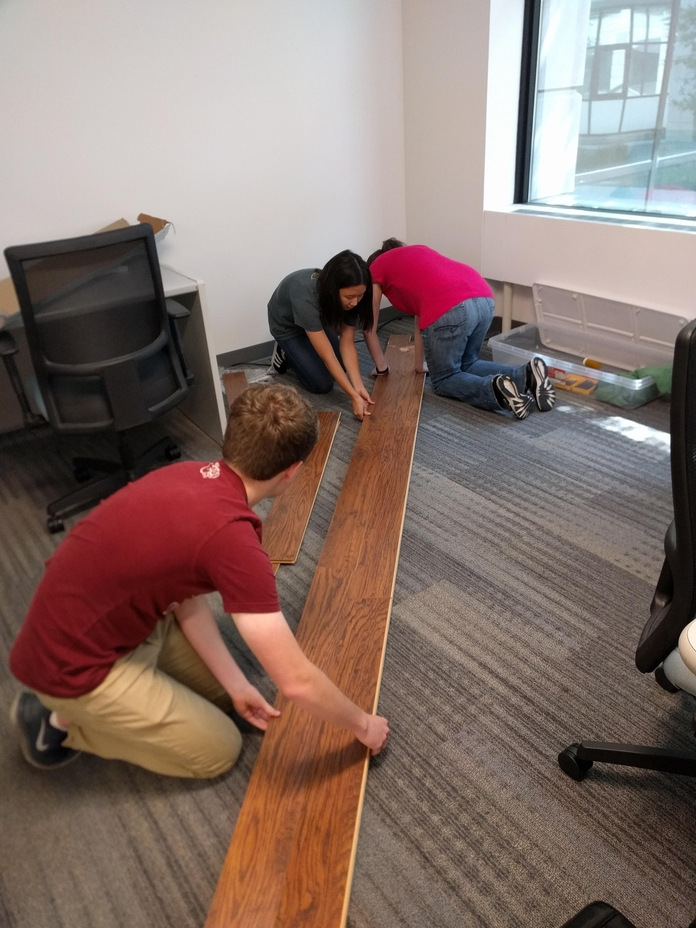
\includegraphics[width=5cm]{Mud_Set}
\caption{Placing the hard wood flooring onto the wooden base.}
\label{Image 1}
\end{figure}

\begin{figure}[!htp]
\centering
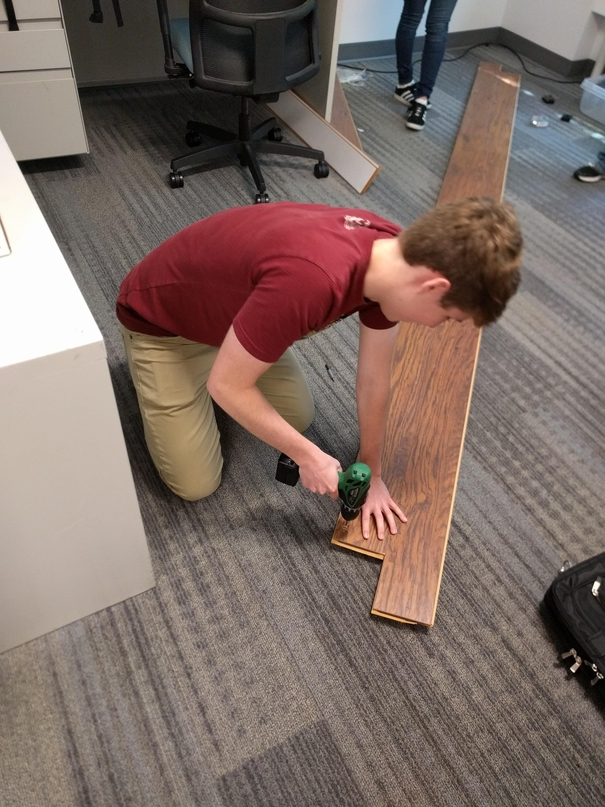
\includegraphics[width=5cm]{Mud_Drill}
\caption{Drilling the hard wood flooring into place}
\label{Image 2}
\end{figure}

\newpage

5. Use an X-ACTO knife to cut any overhanging pieces of wood or linoleum. A table saw may be necessary.


\subsection{Making the Print}

1. For the first trial, scoop 3/4 cup of dirt into a 1-gallon plastic bag (Figure 3). Gently add 300 ml of  water and mix thoroughly.

\begin{figure}[!htp]
\centering
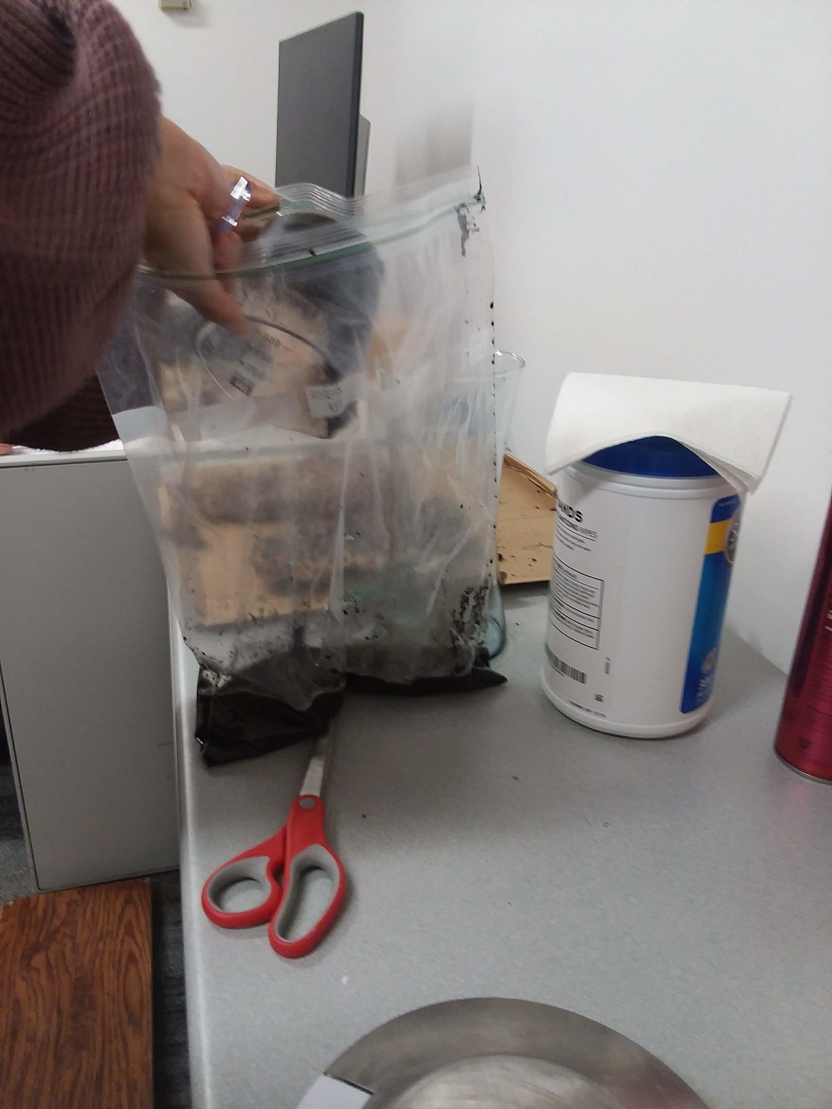
\includegraphics[width=5cm]{Mud_Scoop}
\caption{Portioning out the dirt and water to keep mud consistent across visits. }
\label{Image 3}
\end{figure}

\newpage

2. Pour the mixture into a medium-sized bucket. The liquid should not surpass a height of 1 inch.

3. Lay one vinyl flooring board and one hard wood board side by side on the floor. 

4. Step into the bin and evenly coat the surface of the shoes in muddy water (Figure 4).

\begin{figure}[!htp]
\centering
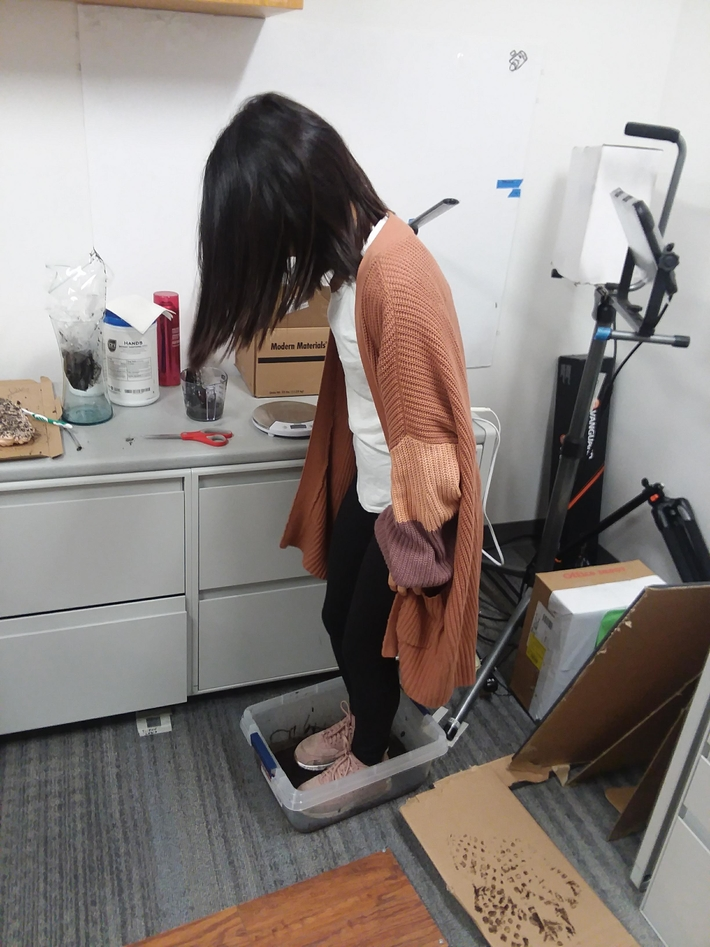
\includegraphics[width=5cm]{Mud_Bin}
\caption{Stepping into the bin of mud. In the case of big shoes, one foot at a time can be placed in the bin. }
\label{Image 4}
\end{figure}

\newpage

5. Step directly onto the linoleum-covered board and take four natural steps (Figure 5).As the person walks, the second technician should move the bin containing mud down to the end of the board.  

\begin{figure}[!htp]
\centering
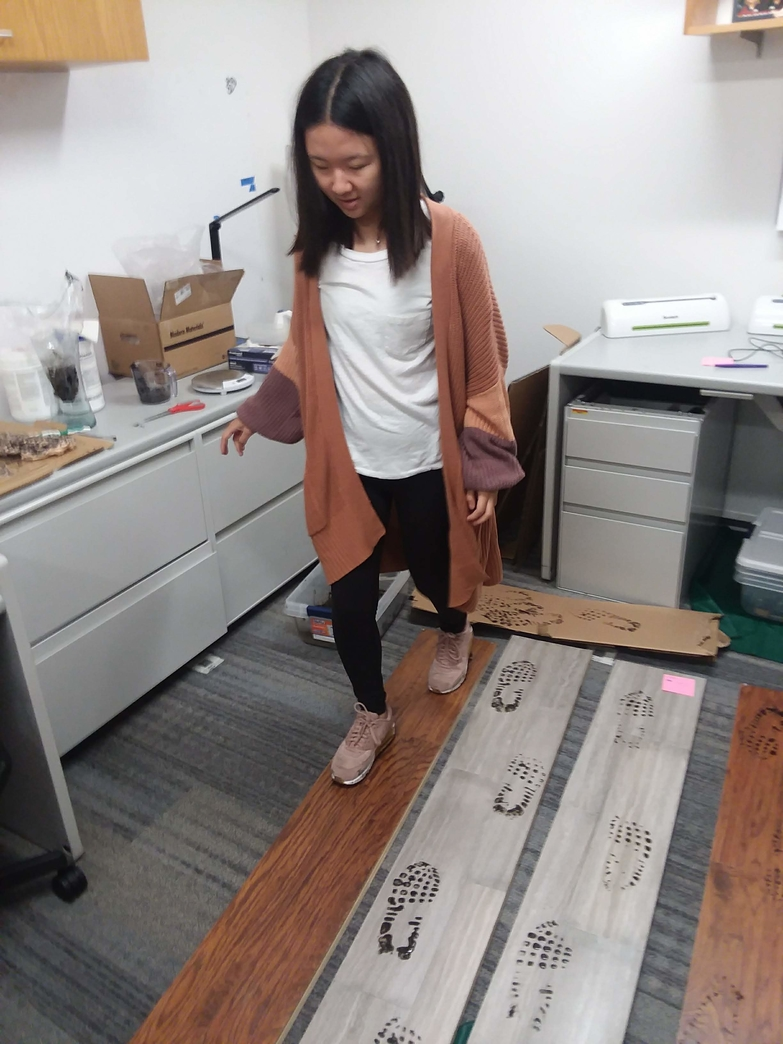
\includegraphics[width=5cm]{Mud_Step}
\caption{Walk down the length of one board with the muddy shoes. }
\label{Image 5}
\end{figure}

\newpage

6. Once across the board, step into the bin to, once again, evenly coat the bottoms of the shoes.

7. Repeat step 5 on the hard wood flooring board.Once across, step onto a piece of cardboard.

8. Take off the shoes and gently hit the shoes together over the bucket filled with mud, making sure that the treads do not contact.

7. Gently rinse off any extra mud in a sink with a soft-bristled brush.

8. For the second trial, scoop 5/8 cup of dirt into a 1-gallon plastic bag. Gently add 150 ml of  water and mix thoroughly.

9. Repeate steps 2-7 for this set of prints. 

9. Allow both sets of prints to dry overnight.


\subsection{Shoe Print Photography}

1. Place the L-shaped ruler next to the shoe print such that the heel of the shoeprint is open.

\begin{figure}[!htp]
\centering
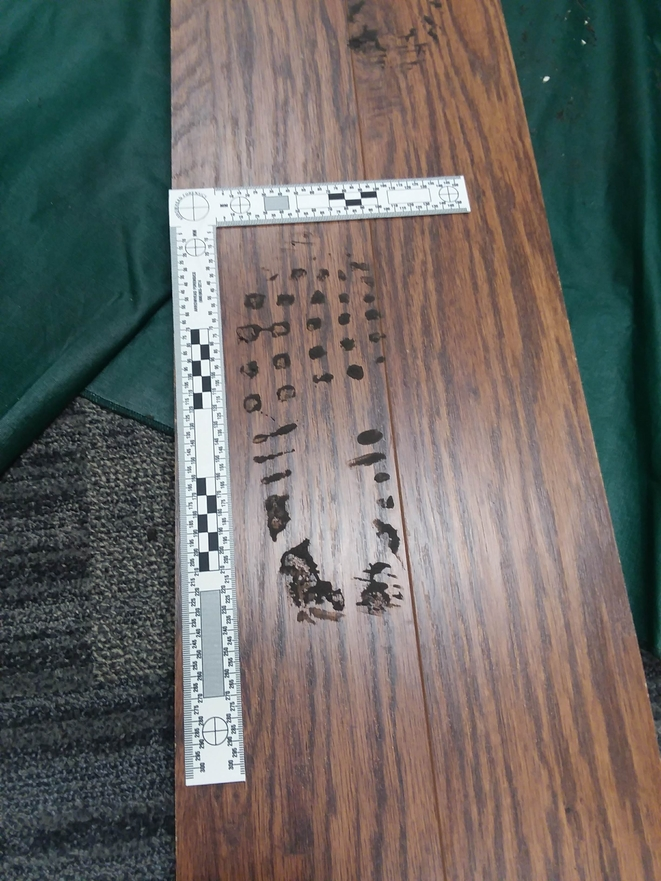
\includegraphics[width=5cm]{Mud_Scale}
\caption{Stepping into the bin of mud. In the case of big shoes, one foot at a time can be placed in the bin. }
\label{Image 4}
\end{figure}

2. Photograph all prints in high definition. Place and level a tripod next to the print. Position the tripod arm about 2 feet above the print. Firmly fasten the camera on to the arm and use a bubble level to level  the arm. It may be necessary to raise or lower certain legs of the tripod to achieve balance. Fasten a counterweight (approximately 8 extra sheets of linoleum flooring in the tripod bag will suffice) along the back of the tripod. Please reference the high resolution photography procedure for exact tripod and camera set-up. 

3.  Locate the attachment point on the end of the tripod arm. Making sure that the counter weight is present on the backside of the tripod, press the orange button and slide the camera into place. There will be a small click when the camera is in place. 

4. Making sure that the camera is turned off, plug the USB cable into the camera body (left side). Do not force the plug or the screw into the camera. Plug the other end into the back of the laptop. 

5. Remove the lens cap and turn on the camera by sliding the switch located on the upper left-hand side of the camera from Off to On

6. The computer currently opens the following:
•	Control panel/hardware and sound/devices and printers/canon EOS 5d mark IV
i.	this window can be closed
•	EOS utility 3
ii.	if this program does not start you can manually start it

7. To remotely take pictures, select “remote shooting”

8. The pop up that comes up is used to control the camera. Select “live view” on this same menu

9. Make sure that the ruler is flat and not covering any portion of the print. 

10. Now, using the live view on the laptop, make sure that the shoe impression and the scale are both present in the shot. If all is visible on the screen, press the acquire button on the main control menu. 

11. Properly name and save the image to the desired folder on the desktop or shared drive. 

12. Take a second image, but this time, utilize the night stick to illuminate the impression from the right side. 

13. Take a third image, but this time, utilize the night stick to illuminate the impression from the left side. At this point, remove the scale and put away the camera and tripod.  
\end{document}

